\documentclass[11pt]{article}
\usepackage{amsmath}
\usepackage{mathtools}
\usepackage{txfonts}
\usepackage[margin=1.0in]{geometry}
\usepackage{graphicx}
\usepackage{float}
\usepackage{booktabs}
\usepackage[caption=true]{subfig}
\graphicspath{ {images/} }
\usepackage{appendix}
\usepackage{url}
%\usepackage{wrapfig}
\usepackage{algorithm}
\usepackage[noend]{algpseudocode}
\usepackage{caption}


\setlength{\parskip}{\baselineskip}%
\setlength{\parindent}{0pt}%
\renewcommand{\baselinestretch}{1.4}

\title{Regression models for predicting rail transit ridership at the station level}
\author{Daniel Hartig}
\date{\vspace{-5ex}}

\DeclareMathOperator*{\argmin}{arg\,min}


\begin{document}
\maketitle
\begin{abstract}
Methods for predicting ridership for future urban rail systems or extensions often have poor accuracy. One study shows that predicted ridership is overestimated by about 50\%, on average, for a broad sample of urban rail systems worldwide.  The ridership estimates produced by most transit agencies in the United States are not based on regression models. This thesis presents a framework for feature generation and regression modeling for estimating urban rail ridership in the  United States.  Features are generated using publicly available data from the US Census Bureau at the zip code level. Monte Carlo geographic sampling from zip code shapefiles generates features for each station on a rail network, representing characteristics within walking distance of that station. Network connections and travel times are used to generate a second set of features representing characteristics within commuting distance of each station. Several models are developed using different regression types and are compared in terms of accuracy and selected features. Some of the generated models provide system-level ridership predictions within 20\% of the true value for a sample set of six US urban rail systems. 
\end{abstract}

\section{Introduction}

The United States is undergoing a rail boom. Since 2010, new light rail lines have opened in Dallas, Los Angeles, Salt Lake City, Denver, Minneapolis, Houston, Seattle and more.  A new heavy rail line opened in Washington DC, and a commuter rail system in Orlando. As transit expands in cities in the United States, there is an opportunity to validate predictive rail ridership models. 

A survey of transit agencies \cite{Boyle2006} conducted by the Transit Cooperative Research Program showed that relatively few agencies are using quantitative models when forecasting ridership for new lines, extensions or stations under consideration for funding. Of the 35 agencies that responded to the survey, 29 use professional judgment and 28 use rules of thumb among one or more techniques used to generate ridership forecasts. Another method used by 22 agencies is service elasticity; a set of general transit demand response curves for changing transportation options, published by the Transportation Research Board \cite{tcrp95}. 

For quantitative methods, the most commonly used technique--by 18 of 35 surveyed agencies--is the four-step travel demand model \cite{McNally2008}, introduced by Mannheim and Florian \cite{Mannheim1979, Florian1988}. The Mannheim-Florian model's four steps are trip generation, trip distribution, mode choice and route choice. In the trip generation phase, trip endpoints are created with production and attraction ends. In the trip distribution step, these endpoints are paired up to generate trips; for example a residence is paired with a job location for one trip, or a hotel is paired with a tourist attraction. In the mode choice step, trips are assigned to various transportation modes, such as personal vehicle, bus, or walking. Finally, in the route choice step, a route using that mode of transportation is chosen.

An implementation of the Mannheim-Florian model can be seen in the Seattle's Sound Transit Ridership Forecasting Methodology Report \cite{ST3_2015, ST3_add}. The Sound Transit 3 (ST3) was a ballot measure that passed in 2016 for a \$54 billion expansion of the local light rail system involving 100 km of new tracks and 37 new stations. The ridership forecasting methodology report explained how the project's official ridership projections were developed. The regional area is divided into 785 Alternatives Analysis Zones and for each of these zones transit surveys and recorded ridership on local bus routes were used to complete the trip generation and trip distribution steps. The mode choice and route choice is done using an incremental logit model to predict changes in transit mode based on changes in transit mode availability.

A significant weakness of the four-step method is that it relies on already known transit ridership \cite{NCTR}. For a proposed light rail system, for example, existing bus routes would be used to complete the trip generation and trip distribution steps.

A regression based ridership model could provide an alternative estimate of ridership without depending on previously known transit ridership counts. Only seven of the 35 surveyed agencies used regression models to predict future transit ridership. This thesis proposes a regression-based model using data from the United States Census Bureau at the zip code level. The model will be trained on the zip code characteristics and ridership data from existing light and heavy rail transit systems. The resulting model will be used to predict ridership on other rail transit systems.  

\subsection{Original Contributions}

There are two main objectives of this thesis. The first objective is to investigate the utility of various data from the US Census Bureau as predictor variables in a regression model for urban rail ridership. The second objective is to determine what generalized linear regression methods--in terms of the choice of loss function and link function--are best suited to modeling urban rail ridership given the available data.

This thesis diverges from previous regression modeling by investigating an expanded set of potential features. The US Census Bureau provides extensive data on a per-zip code bases as detailed in Section \ref{sec:data}: there are over a thousand possible features available. This data is provided as counts per zip code. To translate this zip code data into features for a regression model, this thesis presents a novel geographic sampling method in Section \ref{sec:sampling}. 

With features for regression analysis in hand, this thesis benchmarks several different regression methods. Previous regression based analyses of urban rail ridership have exclusively used ordinary least squares regression. This thesis expands the model base to include other loss functions and link functions and reports accuracy metrics for each model. 

\section{Data Sources and Feature Generation}

\subsection{Selection of Transit Systems}

The response variable for the regression analysis is average weekday ridership over a period of at least one year. Ridership data for agencies that publish annual ridership reports is used to validate the model (for ridership data sources, see Appendix \ref{app:ridership}). Six cities were selected for this study: Boston, Chicago, Los Angeles, Atlanta, Dallas, and Denver. Several cities were eliminated from analysis for various reasons. The author was unable to locate ridership information for several cities such as Houston and Miami. A limitation of the Census dataset is that it does not include government employment. While state level employment is significant in all potential cities, state employment levels are relatively constant from city to city. Federal employment varies greatly, however; Washington DC and San Diego with its military installations had to be eliminated due to the large impact of un-recorded federal employment. San Francisco and Philadelphia were eliminated because they have multiple rail systems without integrated fares. New York City was eliminated because its subway has higher ridership than all other intra-urban rail systems in the country combined.

Ridership data is captured by different methods in different cities, but the same underlying data is counted by each case. In Chicago and Boston, the transit agency measures paid station entries. Boston additionally reports transfers between lines at each transfer station. Therefore, daily ridership is measured as the total number of entrances per station per day. This results in one count per one trip; and two counts per one daily commute. Dallas, Denver and Los Angeles report boarding and alighting by train car; so daily ridership is measured as the total number of boardings per stations per day. For transfer stations, boarding is `double counted' since a boarding at station A and a transfer at station B would result in two counts per one trip. Therefore, for these three networks, the transfer stations and their unusually high ridership counts are excluded from the analysis. For Atlanta, the ridership reporting definition is unknown, so we eliminate the one transfer station as a precaution. For Boston and Chicago, ridership is counted by extracting data from the fare system for paid station entries. In Dallas and Denver, passenger counts are measured at the train car by Automated Personnel Counters. In Los Angeles and Atlanta the counting methodology is unknown. 

The data closest to 2015 is used when possible to get an accurate relation between ridership and census data. The census data as well as Chicago, Dallas, and Denver's ridership statistics are from 2015. Boston's ridership is from 2014, Los Angeles' is from 2013-2014, and Atlanta's is from 2010-2013. 

\subsection{Data Sources for Predictor Variables}\label{sec:data}

The zip code level data for feature generation comes from the US Census Bureau and is available at \texttt{factfinder.census.gov}. There over one thousand potential data sets available. We refer to the data available for each zip code as characteristics of the zip code. Selection of features is guided by Kuby \cite{Kuby2004}, Taylor \cite{Taylor2008}, and Currie \cite{Currie2011}, who demonstrate the significance of characteristics such as employment, population, universities, poverty, airports, park and ride stations, and rental housing units. The characteristics can be divided into two categories: counting characteristics and dummy variables. 

This model emphasizes using only features that have `real' units, as opposed to binary features. The only binary dummy variable this model uses as a feature the presence of park-and-ride parking spaces at a transit station. Instead of using measures of land use mix as proposed in other models \cite{Durning2015, Gutierrez2011}, or binary dummy variables for universities and central business districts, the equivalent information is provided naturally as counting data in the feature set. Counts of housing types (such as large apartment buildings versus single family homes) replace land use mix; the number of jobs at universities or in financial jobs provide more information than dummy variables for presence of universities or central business districts. 

\begin{table}[H]
\centering\begingroup\fontsize{10}{10}\selectfont
\begin{tabular}{ll}
\toprule \textbf{Population related}&\textbf{Employment related} \\ 
\midrule Total population&Total Employment pay\\
Population over age 65& Employment in finance industry\\
Population with bachelor's degree& Employment at hospitals\\
Number of residents employed full time&\\
Number of housing units built after 2000&\\
\bottomrule
\end{tabular}\endgroup
\caption{Examples of characteristics associated with zipcodes}\label{tab:char}
\end{table}

The selected characteristics are generally related either to the population of the zip code or the number of jobs of the zip code. The captured characteristics of the built environment, such as the quantity, age, and building type of the housing stock, are generally related to population. For example, the total number of housing units is expected to be highly correlated with the population of a zip code.  Examples of characteristics are provided in Table \ref{tab:char}. Some characteristics, such as total population, are expected to have a positive relationship with ridership; others, such as population under the age of 18, are expected to have a negative relationship. Examples of associations between characteristics and ridership are provided in Figure \ref{fig:chartypes}. A summary of all the selected characteristics is provided in Appendix \ref{app:features}.



\begin{figure}[H]
\centering
\subfloat[An example of a positive association]{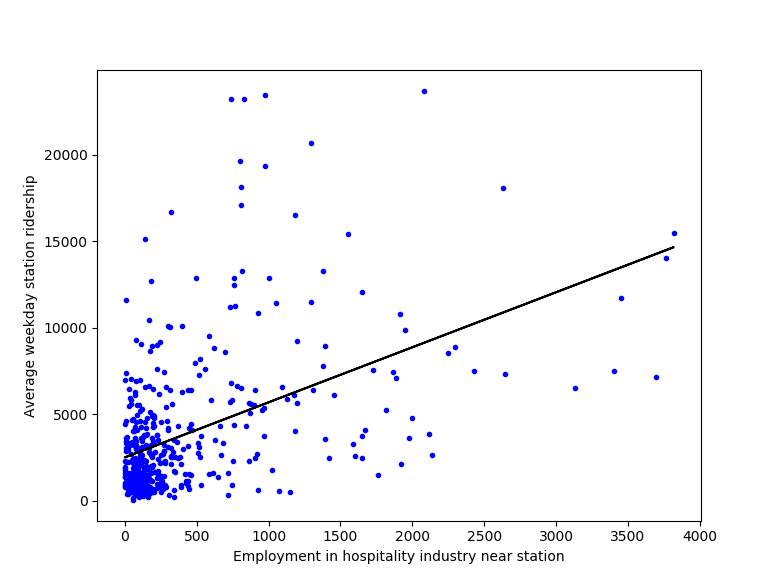
\includegraphics[clip,width=0.5\columnwidth]{exRegPosSlope}}
\subfloat[An example of a negative association]{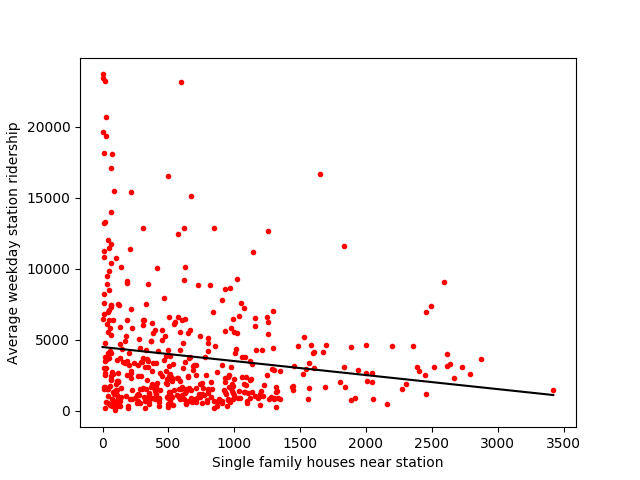
\includegraphics[clip,width=0.5\columnwidth]{exRegNegSlope}}
\caption{Single covariates against the response variable with ordinary least squares (OLS) line of best fit.}\label{fig:chartypes}
\end{figure}


In Yao \cite{Yao2007}, a distinction is made between `Need Index' features, a series of features that depend on the characteristics around the station and are independent of the transit network; and `Transit Network' features, which do depend on the travel time between stations of the transit network. To model network features for each station, the sum of each characteristic for every other station within 15 and 30 minutes transit time is included as a feature of the original station, as described in Section \ref{sec:net}. This provides us a quantitative way to express the 'centrality' dummy variable that is provided as a flag in many models \cite{Kuby2004, Durning2015}. Centrality could be proportional to the count of population or jobs within 30 minutes of a station, for example. 

We translate zip code level data into transit station specific data by sampling each zip code's geographic area to determine proximity to a transit station. For each zip code near the transit network, a set of random points within that zip code is generated using rejection sampling. For each of the those points, one or more closest stations are determined. Each point is assigned to one or more station within walking distance, using the method defined in Section \ref{sec:walk}. Counts for the characteristics of each zip code, such as population or employment, are then assigned to each station proportional to the number of points assigned to each station.

\subsection{Definition of `Walking Distance'}\label{sec:walk}

The area within walking distance of a station is called its `catchment'. To generate a feature for a transit station, the total count of some characteristic within the catchment of that stations is considered. The standard transit catchment distance in literature for rail stations is one half mile (800 m). Guerra \cite{Guerra2012} suggests that one half mile is more appropriate for population as a feature while one quarter mile (400 m) is better for employment as a feature. A case study \cite{ElGeneidy2014} from a 2003 Montreal transit riders origin-destination survey concluded that approximately 50\% of riders of the city's urban rail transit walk less than 500 meters to their stations, while 90\% walk less than 1000 meters. The maximum walking distance is approximately 1500 meters. In another regression-based study of catchment sizes, Gutierrez \cite{Gutierrez2011} found the optimal distance for  for assigning population and employment to a station was between 600 and 900 meters in straight line distance. A straight line distance is measured as the crow flies as opposed to a distance following pedestrian walkways; this distance measurement is consistent with the distances used in this analysis.

A significant concern when tabulating catchments is that in many of the densest regions of cities, there are many stations within a few hundred meters of each other. For example, from the Massachusetts State House in downtown Boston, there are seven urban rail stations on four different train lines within a 10 minute walk, according to Google Maps. Any of those stations could be the `best' place to board and disembark the train for a commute to work at the State House, depending on the direction and train line by which the commuter was arriving in downtown. It is important that we allow some `overlap' in catchment areas; people at one geographic location could use more than one station for various transit needs. 

Given this information, we choose cutoffs of 500 meters and 1000 meters for calculating station distances. For any location that has residents, jobs, or other desired countable characteristics, all stations within 500 meters will be considered equally likely to capture a share of that resident or job's transit demand. If there are no stations within 500 meters; then all stations within 1000 meters will be considered. 

\subsection{Rejection Sampling of Zip Code Shapefiles}\label{sec:sampling}

We translate zip code level data into transit station specific data by using a Monte Carlo method to estimate feature counts near transit stations. Sample points are generated within each zip code near the transit network. Those points are assigned to whichever stations are within walking distance of the station, as defined in Section \ref{sec:walk}. If there are multiple stations within walking distance, then equal fractions of that one point are assigned to each station. The ratio of points assigned to each station to total points generated for each zip code is used to assign feature counts to each station, such that
\[\text{count}(station_i) = \sum_j w_{ij} \cdot \text{count}(zipcode_j)\]
where $w_{ij}$ is the proportion of the points generated in zipcode $j$ that are assigned, wholly or partially, to station $i$. Not all areas within a zip code $j$ will be within walking distance of any station $i$, so 
\[\sum_j w_{ij} \leq 1\] for all $j$. An algorithm for rejection sampling a single zipcode is provided in Algorithm \ref{alg:rejsamp}.


\begin{algorithm}\begingroup\fontsize{10}{10}\selectfont
\begin{algorithmic}
\State{ Given \texttt{zipcode} is a single zipcode near the transit network }
\State{ Let \texttt{zipcode.latrange} and \texttt{zipcode.lonrange} be maximum and minimum latitude or longitude for \texttt{zipcode} shapefile}
\State{ $n\gets$ max(\texttt{zipcode.area} in hectares, 1000)}
\State{ \texttt{randomPoints}$ \gets \{\}$}
\While{ len(\texttt{randompoints}) $< n$}\Comment{Generate \texttt{n} random points within \texttt{zipcode}}
	\State{\texttt{lon }$ \gets $ random number $\in$\texttt{ zipcode.lonrange}; \texttt{lat} $ \gets $ random number $\in$\texttt{ zipcode.latrange}}
	\State {\texttt{point }$ \gets$ (\texttt{lat, lon})}
	\If { \texttt{point} is inside \texttt{zipcode.shapefile} and \texttt{point} is not inside exclusion areas}
		\State{ \texttt{randomPoints }$ \gets$ \texttt{randomPoints }$\bigcup$\texttt{ point}}
	\EndIf
\EndWhile
\For{ \texttt{point} $\in$ \texttt{randomPoints}}\Comment{Assignment of points to stations}
	\State{ $n_{0.5} \gets$ number of stations within 0.5 km of \texttt{point}}
	\State{ $n_1 \gets$ number of stations within 1 km of \texttt{point}}
	\If{ $n_{0.5} > 0$}
		\For{ \texttt{station} within 0.5 km of \texttt{point}}
			\State{\texttt{station.characteristicValue }$  \mathrel{+}= $ \texttt{ zipcode.characteristicValue}$\, / \,n_{0.5}$} 
		\EndFor
	\ElsIf {$n_1 > 0$}
		\For{ \texttt{station} within 1 km of \texttt{point}}
			\State{\texttt{station.characteristicValue }$  \mathrel{+}= $\texttt{ zipcode.characteristicValue}$\, / \,n_1$}	
		\EndFor
	\EndIf
\EndFor
\end{algorithmic}\endgroup\caption{Algorithm for estimating characeristic counts that are near transit stations}\label{alg:rejsamp}
\end{algorithm}



The US Census Bureau provides TIGER/Line shapefiles of each zip code tabulation area (ZCTA) in the United States at \url{https://www.census.gov/geo/maps-data/data/tiger-line.html}. Random points are generated in a rectangular box drawn around the extremities of each zipcode's shape; these random points are accepted if they are within the shapefile or rejected if they are outside it. Those points that are inside the shapefile are tested against author-created exclusion zones. These zones are shapes within the zip code's shapefile area that are known to not have any population, employment, or other countable characteristics. The exclusion zones are mostly drawn over water areas and parks. Those points that are inside the exclusion zones are also rejected. This creates a set of points randomly drawn from the zip code's land area, not counting unoccupied regions like parks. 

The set of points is tested for their distance to any transit stations to determine which station catchments they fall in, as described in Section \ref{sec:walk}. The characteristic counts associated with each tested point are divided between all stations within 500 meters. If there are no stations within 500 meters, then the point is divided between all stations within 1000 meters. If no stations are within 1000 meters, that point is not assigned to any station. The total sum of points and fractional points assigned to each station is divided by the total points available to get the fraction of each of the zip code's characteristic data counts is assigned to that transit station. 

\begin{figure}
\begin{center}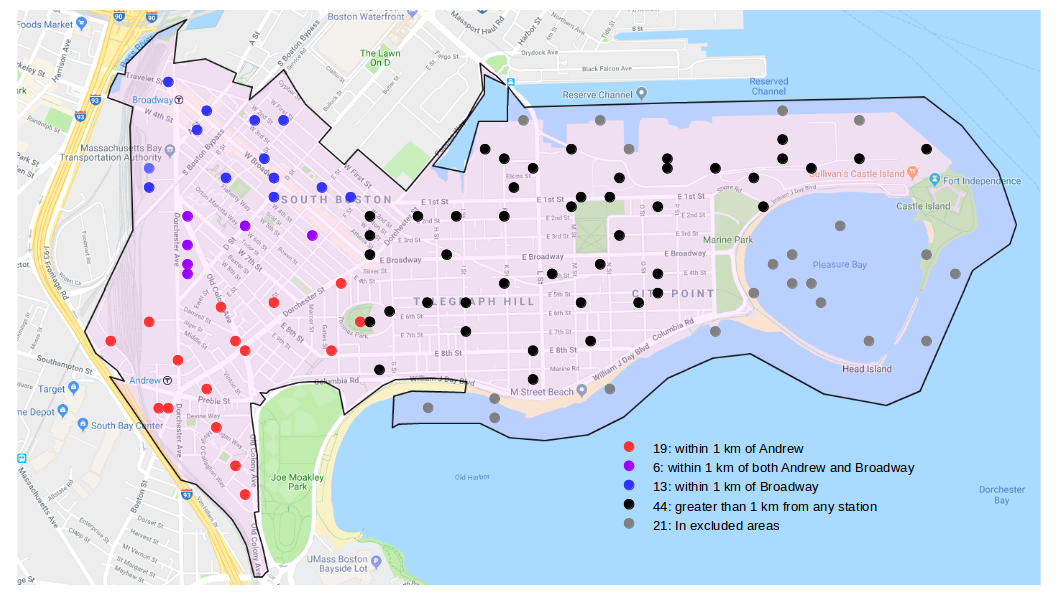
\includegraphics[scale=0.55]{geo_point_demonstration}\end{center}\caption{Illustration of nearest zip code estimation for zip code 02127.}\label{fig:f1}
\end{figure}


An example using zip code 02127, the South Boston neighborhood of Boston, illustrates the sampling method (Figure \ref{fig:f1}). 100 random points are selected within the area of the shapefile. Of these, 21 points indicated in gray are rejected due to exclusion areas based on water area, parks and abandoned port facilities. Of the remaining 79 points, 8 are within 500 meters of Andrew station, while 6 are within 500 meters of Broadway station. Moving out to the 1000 meter radius, 11 are within 1 km of Andrew station, for a total of 19 that are close to Andrew; 7 are within 1 km of Broadway station for a total of 13 that are close to Broadway; and 6 are within 1 km of both. The 6 points within 1 km of both stations are divided evenly between the two. The total population of South Boston is 36494. Therefore, 
\begin{align*}
\text{Counts assigned to station} &= \frac{\text{\# points for one station} \cdot \sum\frac{\text{\# points for multiple stations}}{\text{\# stations for each point}}}{\text{\# points for zipcode}}\cdot\text{characteristic counts}  \\
&= \frac{19 + \frac{6}{2}}{79}\cdot 36494 \text{ people} \\
&= 10163 \text{ people}
\end{align*}
are assigned to Andrew station. Similarly, 7391 people are assigned to Broadway station. Summed over all zip codes near Andrew and Broadway stations, this shows how the total population within walking distance of the station is estimated. This calculation is performed for all countable features and all zip codes and summed total counts for each characteristic are used as a feature for each transit station. 

\subsection{Variance of Monte Carlo estimates}

With any Monte Carlo method for estimation, there is variance in the estimates generated. In this case, the variance comes primarily from the random locations of the points. It is possible that in different Monte Carlo trials, a station may get significantly more or less points nearby it. This is especially significant in areas of high population density; one extra or missing point could be worth hundreds or thousands of jobs in the densest areas of downtown Chicago or Boston. To keep variance to an acceptably low level, we must generate enough sample points that variation between trials is minimal. 

The number of points that will be accepted by rejection sampling is set beforehand. We generate random points, and use rejection sampling to see if they are inside the shape of the zipcode and outside of any exclusion zones. We continue generating points until we have reached the desired number of accepted points.

The land area of the zip codes near the studied transit networks vary in size from as small as 30 hectare in downtown Chicago to as much as 18100 hectares at the suburban end of transit lines in Dallas. To provide an appropriate balance between accuracy and processing speed, we use one accepted point per hectare, but with a minimum limit of 1000 accepted points per zip code. This effectively provides over 10 points per hectare in for the zip codes in the densest parts of the studied networks: the downtown areas of Chicago and Boston. These areas also have the densest network of transit stations, with many stations within a kilometer of each other. In these denser areas, it is important to have enough points that the division of points between stations does not result in too much variance. 

We generate 100 sets of estimates for the a single feature (total population) for all stations in the six transit networks. Figure \ref{fig:mcvar}(a) shows a graph of means of total population estimates against standard deviation of the population estimates, while Figure \ref{fig:mcvar}(b) is means against coefficient of variation. The standard deviation shows an increasing linear relationship with the population mean. The coefficient of variation is never greater than 10.4\% and generally decreases with increasing estimated mean population. The mean coefficient of variance over all studied stations is 5.3\%. By this method, the relative accuracy of any single station estimate of population or employment relative to the mean of 100 estimates of the same feature $\pm$10\% .

\begin{figure}[H]
\centering
\subfloat[Standard deviation versus mean by transit station.]{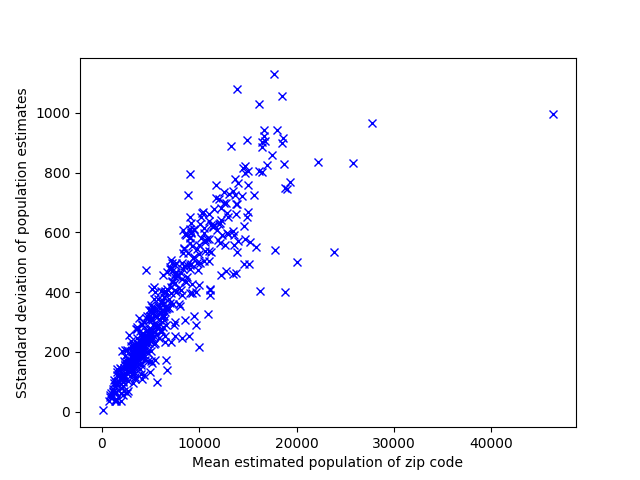
\includegraphics[clip,width=0.5\columnwidth]{estvarstdev}}
\subfloat[Coefficient of variation versus mean by transit station.]{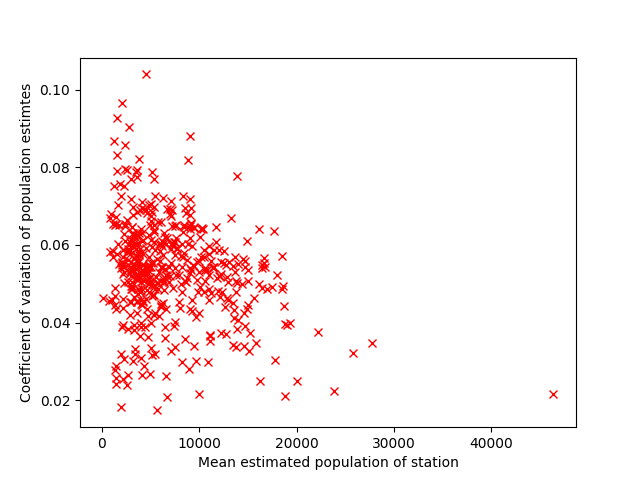
\includegraphics[clip,width=0.5\columnwidth]{estvarcov}}
\caption{Indications of variance for Monte Carlo estimates of the population feature.}\label{fig:mcvar}
\end{figure}

\subsection{Generation of network-dependent features}\label{sec:net}

For each `Need Index' type feature generated by rejection sampling, a set of corresponding network-based features are generated to represent the sum total of a certain characteristic (such as population or employment) within a given travel time of that station. An algorithm for calculating network characteristics is shown in Algorithm \ref{alg:network}. 

\begin{algorithm}
\begin{algorithmic}
\For{\texttt{station}$ \in$ transit network}
	\State\texttt{nearby15} $\gets$ all other stations within 15 minutes travel time of $station$
	\State \texttt{nearby30}$ \gets$ all other stations within 30 minutes travel time of $station$
	\For{every characteristic in the model}
		\For{\texttt{otherStation} $\in$ \texttt{nearby15}}
			\State{\texttt{station.characteristicValue15} $+=$ \texttt{otherStation.characteristicValue}}
		\EndFor
		\For{\texttt{otherStation}$ \in$ \texttt{nearby30}}
			\State{\texttt{station.characteristicValue30} $+=$ \texttt{otherStation.characteristicValue}}
		\EndFor
	\EndFor
\EndFor
\end{algorithmic}\caption{Algorithm for calculating network characteristic counts}\label{alg:network}
\end{algorithm}

The transit network is laid out as a directed graph, where nodes represent the transit stations and edges are weighted by the travel time between the stations. Travel times between stations are available in the transit schedules published by the appropriate transit agencies. Travel times can be different in different directions, following the published schedules. At transfer points, there is a separate node for a single station on each line. The multiple nodes for the same station have edges between them weighted by the average wait time between trains. The wait time is estimated at half the time between trains at the station being transferred to. For example, if one train arrives every 10 minutes, then a transfer to a node on that line at any station will have an estimated travel time of 5 minutes. Many transit agencies align arrival times so that one line will depart a few minutes after another train arrives. No attempt is made to capture this more complicated arrangement of estimated transfer times. 

\begin{figure}
\begin{center}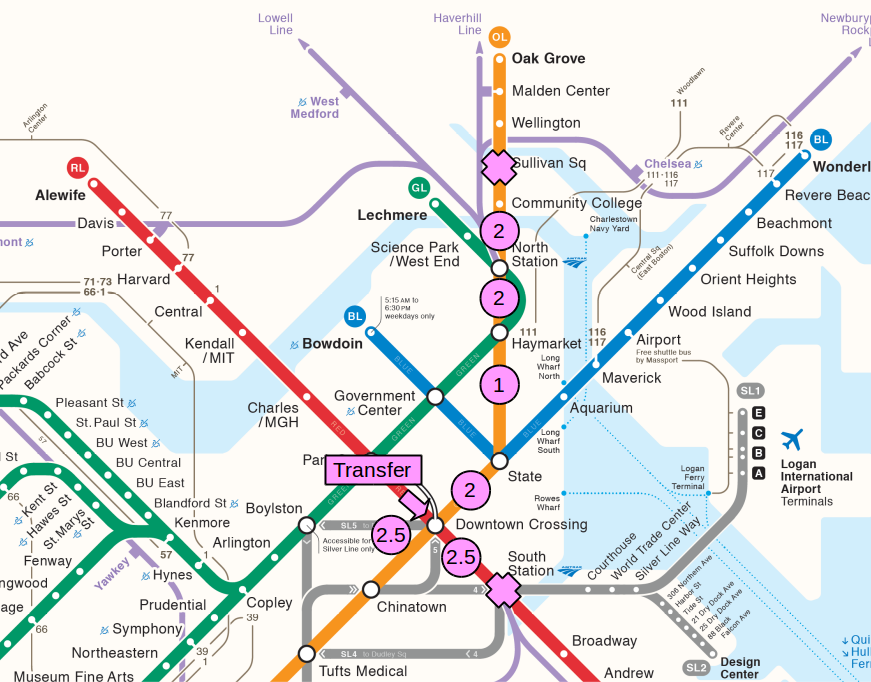
\includegraphics[scale=0.7]{transfer_demonstration}\end{center}\caption{Illustration of travel time calculation for Sullivan Square to South Station, in Boston.}\label{fig:f2}
\end{figure}

An illustration of the calculation of travel time between Sullivan Square and South Station in Boston is provided in Figure \ref{fig:f2}. Starting at Sullivan Square on the Orange Line southbound, there are four edge traversals totaling seven minutes to get to Downtown Crossing. From there, there is a 2.5 minute wait until a Red Line (also Southbound) train arrives, and 2.5 more minutes of travel to South Station. The total travel time is thus twelve minutes. 

For any given station, we find a set of all stations within aX distance by selecting an ego graph out of the entire transit network. An ego graph is a sub-graph containing all nodes that are within a specified distance of the central node. 

For each station $A$ and for the set of all stations ($S$) within 15 minutes of $A$; the counts of each `Need Index' type feature is summed over all stations of $S$. This is the count used for the corresponding network type feature of $A$. The same procedure is repeated for all stations within 30 minutes of $A$. Thus, for each `Need Index' type feature associated with a station in the feature set, there are two additional features: one summing the counts of that feature within 15 minutes and one within 30 minutes.

These features are important for providing a measure of centrality to the network. Stations near the center of the network and at transfer points between lines will have higher counts of network features than peripheral stations. The other important function of the network features is to provide estimates of the total scale of system ridership. The more people, jobs, and other characteristics near transit stations, the higher the overall system ridership is expected to be. This is a key component of the model's portability between different city's transit networks. 

\subsection{Analysis of zip code characteristics by city}
%\vspace{-15pt}
\begin{figure}
\centering
\subfloat[Boston - Blue; Chicago - Red; Los Angeles - Green]
{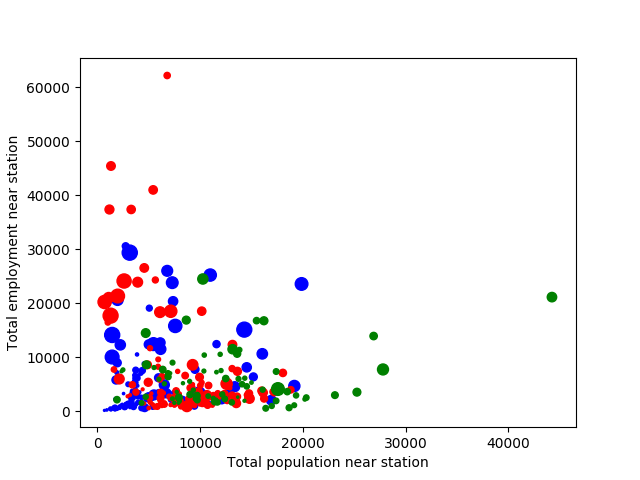
\includegraphics[clip,width=0.8\columnwidth]{localvars_large}}

\vspace{-15pt}
\subfloat[Atlanta - Blue; Dallas - Red; Denver - Green]{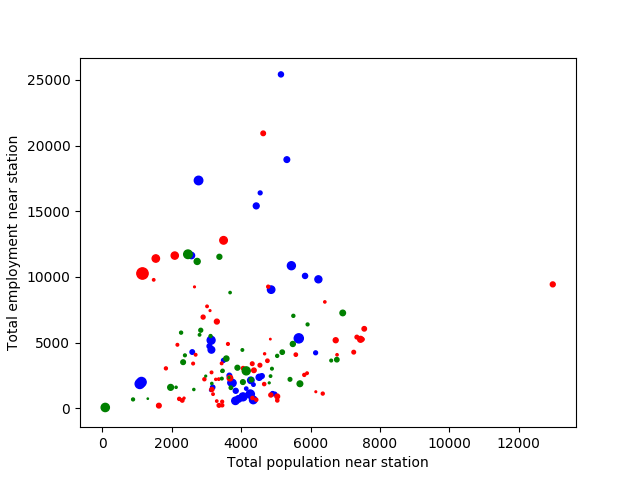
\includegraphics[clip,width=0.8\columnwidth]{localvars_small}}
\captionsetup{singlelinecheck=off, justification=centering}
\caption[]{Employment against population with a 15 minute transit ride for sets of three transit networks.\linebreak
Area of marker represents ridership of the station}\label{fig:localvars}
\end{figure}

The purpose of including multiple transit networks with varying levels of ridership is to ensure that the model captures a broad range of relationships between employment, population and other zip code characteristics on the one hand, and transit ridership on the other. Figure \ref{fig:localvars} shows the employment and ridership counts within walking distance assigned to each station on the transit networks. The ridership of each stations is proportional to the area of the marker for each station. We can see that there is a wide range of population and employment figures near transit stations. In our selection of six transit networks, some networks have much higher peaks of certain zip code characteristics than others, so the graphic is divided into two subfigures, one for the higher ridership networks and one for the lower. 

Station remoteness has a significant impact on the characteristics of stations. For example, the five highest population transit stations are all in Los Angeles. It is not true that the densest areas of Los Angeles have a higher population density than Boston or Chicago. Rather, the Los Angeles transit network has lower station density than Boston or Chicago in the areas of highest population density. Therefore, some stations in high population density areas of Los Angeles will have a transit catchment of up to two square kilometers. For Boston or Chicago, with closer station spacing and multiple lines, any point in the areas of highest population density will have four or more stations within walking distance.  

\begin{table}
\centering\begingroup\fontsize{10}{10}\selectfont
\begin{tabular}{l|cccc}
\toprule Network City&Total Population&Total Employment&Network length (km)&Avg Weekday Ridership \\ 
\midrule Chicago&1189454&872206&157&608472\\
Boston&622484&656375&98&591823\\
Los Angeles&935041&436846&169&254183\\
Atlanta&150171&207601&77&150237\\
Dallas&255092&261813&150&96069\\
Denver&161542&170631&149&75128\\
\bottomrule
\end{tabular}\endgroup
\caption{Network wide characteristics for the six transit networks considered in this thesis}\label{tab:netsize}
\end{table}

The overall characteristics of each transit network are found in Table \ref{tab:netsize}. There is a positive linear relationship between both population and employment and ridership at the network-wide level. However, the effect of network length is also significant. For example, Atlanta's population and employment near its transit stations are both lower than that of Dallas, but Atlanta's ridership is fifty percent larger. Atlanta's network length is about half that of Dallas, suggesting that Atlanta's transit accessible population and employment are compressed into a much smaller area. This density appears to be a significant factor in Atlanta's higher ridership. However, looking at Figure \ref{fig:localvars}(b), where Atlanta's stations are in the blue and Dallas' in red, it is not clear that Atlanta's stations have any individual advantage in population and employment. 

This shows the necessity of the network-dependent features. In Figure \ref{fig:networkvars}, we see the sum of population and employment within a 15 minute transit rider of each station, instead of within walking distance of each station. In Figure \ref{fig:networkvars}(b) we see that Atlanta's smaller network and more tightly spaced stations means that stations generally have more other stations within a given travel distance. Therefore, many of Atlanta's stations have higher network population and employment counts than their corresponding stations in Dallas. The inclusion of the network features will allow the regression model to more accurately predict the higher ridership for stations in Atlanta. 


\begin{figure}
\centering
\subfloat[Boston - Blue; Chicago - Red; Los Angeles - Green]
{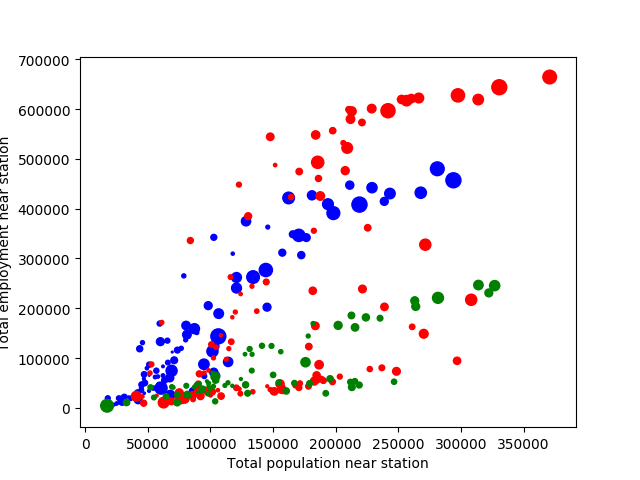
\includegraphics[clip,width=0.8\columnwidth]{networkvars_large}}

\vspace{-15pt}
\subfloat[Atlanta - Blue; Dallas - Red; Denver - Green]{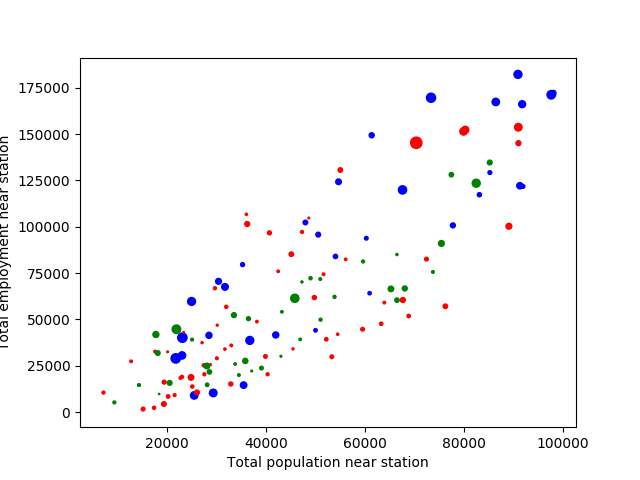
\includegraphics[clip,width=0.8\columnwidth]{networkvars_small}}
\captionsetup{singlelinecheck=off, justification=centering}
\caption[]{Employment against population with walking distance for sets of three transit networks.\linebreak
Area of marker represents ridership of the station.}\label{fig:networkvars}
\end{figure}


\section{Model generation and Error Metrics}

\subsection{Metrics for assessing accuracy of predictions}\label{sec:metric}

In general, the projected ridership forecasts of new transit infrastructure investments significantly overestimates transit ridership. The pioneering study in this field by Pickrell in 1989 \cite{Pickrell1989} found that for ten rail projects completed between 1977 and 1985, and assessed between 1986 and 1989, the actual ridership was between 28\% and 85\% lower than projected. A 2006 study \cite{Flyvbjerg2006} of 25 major passenger rail projects in 14 nations found that 21 of the projects had actual ridership below projections, with the average true system ridership 48\% below the projection. Accurate assessment of projection accuracy is imperative for creating ridership estimates that serve the public interest.

To assess the predictions from regression analysis, there should be two metrics used: one for the total system ridership, and another for station level ridership. The economic justification for new construction of a transit system is based on projections of total system ridership. The projected cost of operating the system must be proportional to the projected revenue from ridership. The placement of stations should be guided by an evaluation of station level ridership. Decisions on whether to fund infill stations along existing transit lines, or line extensions to previously unserved areas depend on analysis of ridership at the station level. Therefore, it is important to create a ridership model that optimizes both system and station level ridership. 

Following Pickrell, the metric for system-wide projection accuracy is standard percentage error in total system ridership, which we will refer to as system error. This error is
$$E_{system} = \dfrac{\left|\,\sum\limits_{i\,\in\,\text{stations}} y_{i, proj} - \sum\limits_{i\,\in\,\text{stations}} y_{i, true}\,\right|}{\sum\limits_{i\,\in\,\text{stations}} y_{i, true}},$$
where $y_{proj}$ is the projected ridership and $y_{true}$ the true ridership for each station, and each is summed over all stations in a transit network.

Hardy \cite{Hardy2010} extends Pickrell's analysis by including absolute station error for stations on newly added sections of an existing transit network. Following Hardy, a measure of station level error on a network is the summed absolute error of all station projections. The rail networks in this study vary widely in total ridership; therefore, to allow network-to-network comparison, this summed absolute station error can divided by total system ridership. The resulting metric for station error given a projected ($y_{proj}$) and actual ridership ($y_{true}$) is 
$$E_{station} = \dfrac{\sum\limits_{i\,\in\,\text{stations}}\left|\,y_{i, proj} - y_{i, true}\,\right|}{\sum\limits_{i\,\in\,\text{stations}} y_{i, true}}.$$

We refer to this metric as station error. 

\begin{figure}
\centering
\begin{minipage}{0.45\textwidth}
\centering
\subfloat[Ridership against population. Linear regression in red, log regression in blue.]{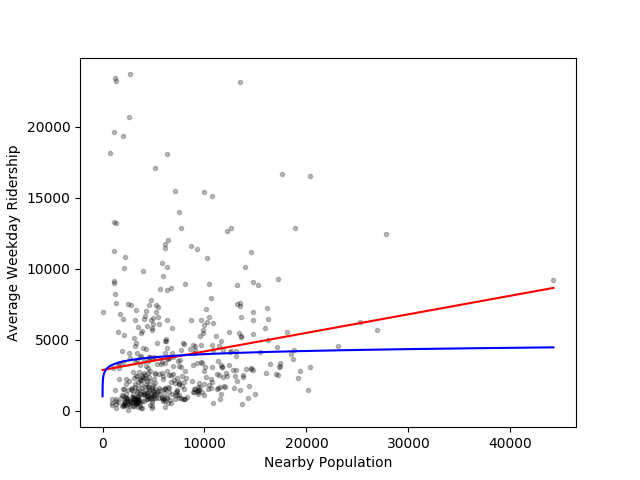
\includegraphics[clip,width=\columnwidth]{popvrider}}

\subfloat[Residual from linear regression against population]{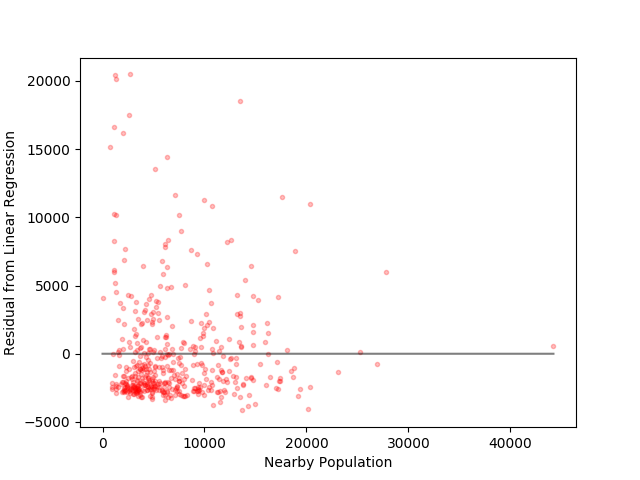
\includegraphics[clip,width=\columnwidth]{poplinresid}}

\subfloat[Residual from log regression against population]{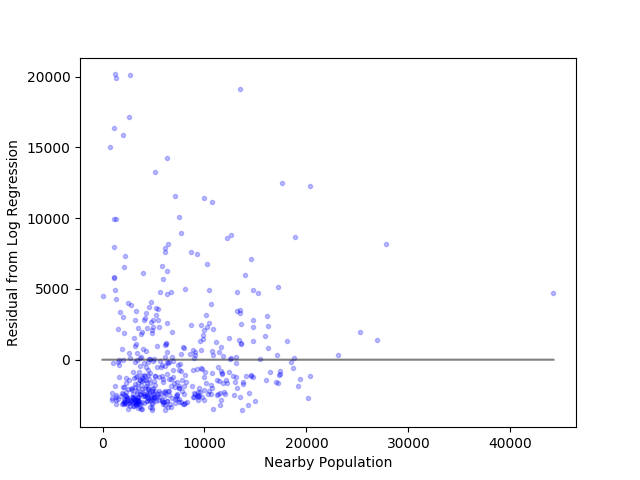
\includegraphics[clip,width=\columnwidth]{poplogresid}}
\caption{Analysis of population regression}\label{fig:popresid}
\end{minipage}\hfill
\hspace{5pt}
\unskip\vrule
\hspace{5pt}
\begin{minipage}{0.45\textwidth}
\centering
\subfloat[Ridership against employment. Linear regression in red, log regression in blue.]{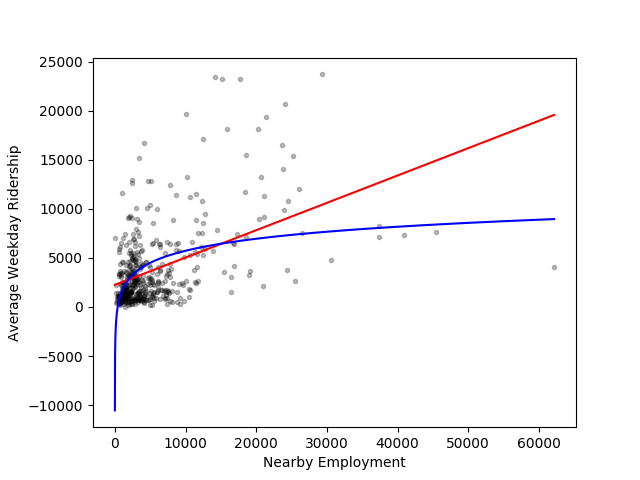
\includegraphics[clip,width=\columnwidth]{empvrider}}

\subfloat[Residual from linear regression against employment]{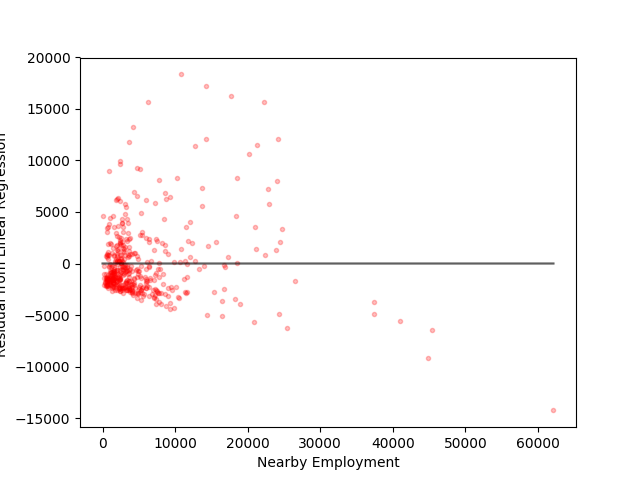
\includegraphics[clip,width=\columnwidth]{emplinresid}}

\subfloat[Residual from log regression against employment]{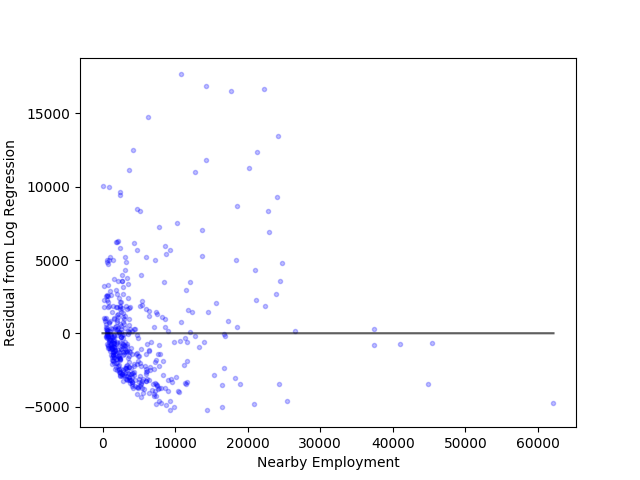
\includegraphics[clip,width=\columnwidth]{emplogresid}}
\caption{Analysis of employment regression}\label{fig:empresid}
\end{minipage}\hfill
\end{figure}


\subsection{Data distribution and regression selection}

Regression models for station level ridership have used ordinary least squares regression \cite{Kuby2004, Taylor2008, Currie2011, Durning2015, Gutierrez2011} to generate predictions. We investigate the applicability of more complex regression models, and whether or not these other regression types can provide better modeling accuracy.

The dependent variable, average weekday ridership at a station, has range $[0, \infty)$. The exponential function has this range and so it is reasonable to assume that there may be a logarithmic relationship between characteristics and ridership. We can compare a linear least squares line of best fit with a line of best fit using the logarithm of the ridership as the response variable. 

There are generally two types of feature included in this survey: those that are related to population and those that are related to employment. A plot of all stations' population versus ridership appears in Figure \ref{fig:popresid} with linear and logarithmic regression lines and residuals. A similar treatment for employment versus ridership appears in Figure \ref{fig:empresid}. In Figures  \ref{fig:popresid}(a) and \ref{fig:empresid}(a), a linear and logarithmic best fit line are fitted to the data. The residuals from the linear regression line are plotted in (b) and from the logarithmic regression in (c) of each figure. 

The coefficient of determination for the two regression types for both population and employment are shown in Table \ref{tab:regr2}. Judging from the coefficients of determinations and the distributions of the residuals, there does not appear to be any clear modeling advantage from using either a linear or log transformed response variable.

\begin{table}[H]
\centering
\begin{tabular}{lcc}
\toprule Variable&Linear R$^2$&Log R$^2$ \\ 
\midrule Population&0.0267&0.0034 \\
Employment&0.1948&0.1878 \\
\bottomrule
\end{tabular}
\caption{Regression of Population and Employment against ridership}\label{tab:regr2}
\end{table}


The metrics for projection accuracy introduced in Section \ref{sec:metric} depend on the absolute difference between actual and predicted ridership. This suggests that regression using the Least Absolute Deviation (LAD) (\ref{sec:lad}) loss function is appropriate for this problem. Since the response variable (ridership) has a value of integer counts, and the variance of ridership increases with increasing employment, we will also investigate the use of a Poisson model. Finally, we will use ordinary least squares (OLS) regression as a baseline comparison, to see if the other methods have any performance advantage compared to the currently used regression type. To test a variety of transformed relationships between the features and response variable, we will test the Poisson regression with both the log and identity link functions, and least squares regression with both a linear response variable and a log-transformed response variable.

Upon performing any regression analysis, it becomes immediately apparent that one set of features is different from the others. Estimating station ridership using only the number of post-secondary (college-level) students within a 15 or 30 minute transit trip of each station provides a very accurate measurement of system level ridership. These variables are represented in the model as \texttt{15net\_students} and \texttt{30net\_students}, respectively. We show the results of a single variable OLS regression of the one variable against ridership. The scores are the average of the six way cross-validation across the six transit networks in the study; each of the six networks is used as the test set in one case, while the other five transit networks are used as the training set. The `best' scoring other feature (\texttt{15net\_hunits\_old}; the number of housing units built before 1940 within a 15 minute transit ride) is shown for comparison.

\begin{table}[H]
\centering
\begin{tabular}{lcc}
\toprule Variable&System Error&Station Error\\
\midrule 30net\_students&0.1016&0.5961\\
15net\_students&0.0946&0.6197\\
15net\_hunits\_old&0.2854&0.6700\\ 
\end{tabular}
\caption{Error for single variable OLS for selected features}\label{tab:students}
\end{table}

The system error scores for \texttt{30net\_students} and \texttt{15net\_students} are much lower than for any other variable, while the station error for these features are also lower than any other features. As we will see, the single-feature OLS of either of these features produces a model that is approximately as good as any other model we will develop. This raises questions about the relationship between this feature and the response variable. It is possible that the population of students within walking distance of a transit station is driven by the availability of local transit, and not the other way around; that is, students may choose their housing locations based on availability of transit. In that case, the number of students is not a valid explanatory variable. Since the relationship is unclear and these features are outliers, we will remove all features derived from number of post-secondary students from the model.

There are 94 remaining features, while some transit networks have as few as 38 stations. Feature selection is necessary to prevent the model from being over-specified. We use two methods of feature selection for each of the five regression types: LASSO regression described in Section \ref{sec:lasso} and a stepwise forward selection method described in Section \ref{sec:fs}. 

\subsection{Feature Selection}

\subsubsection{Feature selection by LASSO regularization}\label{sec:lasso}


Least Absolute Shrinkage and Selection Operator (LASSO) regression can be used to perform feature selection for regression analysis. The LASSO method adds a regularization term to an objective function to penalize regression coefficients. By forcing the sum of the absolute values of all regression coefficients to be less than a fixed value, some regression coefficients are set to zero, thereby eliminating them from the model. 

Because LASSO constrains the magnitude of the coefficients, it is important that all coefficients are on the same scale. Therefore, for all LASSO feature selection methods, the features are normalized by z-score standardization. Each entry $x_{i,j}$ in the covariate matrix is scaled by
$$ x_{i, j, scaled} = \frac{x_{i,j} - \mu_i}{\sigma_i}$$ where $\mu_i$ and $\sigma_i$ are the mean and standard deviation of the $i$-th column of the covariate matrix.

An important part of the LASSO solution is selection of $\lambdaup$, the penalty coefficient. The derivation of the LASSO optimization equations are described in each subsecetion of Section \ref{sec:derive}. The penalty in a LASSO regression is divided into two parts: a loss function on the error of the predicted values and a penalty on the regression coefficients. For a sufficiently large value of $\lambda$, the optimum solution is for all regression coefficients to be zero, thus eliminating the regression coefficient penalty. Solving for the optimum $\lambda$ thus requires identifying the minimum $\lambda$ value for which the solution is all zero coefficients, a solution with zero degrees of freedom. This is typically done by a grid search; this is the method used by the \texttt{glmnet} package \cite{friedman2010}. From \texttt{glmnet}, we use the cross-validation methods that will automatically optimize $\lambda$. The minimum value of $\lambda$ where the solution has zero degrees of freedom is identified by grid search, and then cyclical coordinate descent is used to find the optimum $\lambda$ value. 

LAD LASSO is performed using the \texttt{flare} package in R; this package does not have a built in cross-validation algorithm to optimize $\lambda$. Instead, the author created a $\lambdaup$ grid search algorithm comparable to that performed by \texttt{glmnet}. The Poisson LASSO with identity link is performed by author supplied code, where $\lambdaup$ is solved concurrently with the regression parameters ($\theta$) by an interior point solver, as detailed in section \ref{sec:poiss}.

LASSO regression is performed six times for each LASSO regression type. A trial is made with each city as the test set and all other cities as the training set. Therefore, we identify six sets of selected features for each LASSO regression type. To choose a single set of features from these six sets, we choose all features that are selected by four or more of the six cross-validation trials. This is the feature set that will be reported in the results section.

\subsubsection{Feature selection by stepwise forward selection}\label{sec:fs}
 
Since the data set for this problem is small--with only 466 total stations--we can validate the LASSO results using a stepwise forward selection approach. This method is a greedy search of all possible features to find the best combination of features that minimizes our error metrics, performed in a multi-step process. This process is performed for each of the five regression types defined in Table \ref{tab:regtype}. 

In the first step, for all features, we perform a single-covariate regression against the response variable: ridership. Each feature is evaluated in six-way cross validation, where each of the six transit networks is used as the test set once, while the other five are used for the training. Since there are two types of error defined in Section \ref{sec:metric}, station and system error, we use the arithmetic mean of the two error metrics to score each feature. We then take the arithmetic mean of the score from all six trial runs, and select the single feature with the lowest error score. If $k$ represents one of the six systems that is evaluated as the test set, then the error score for each feature is

$$ E_{feature} = \displaystyle\frac{\sum\limits_{k\in 6\,systems}\displaystyle\frac{E_{k, system} + E_{k, station}}{2}}{6}.$$

After choosing a feature in the first step, in the second step we perform a two covariate regression against ridership. The feature selected in the first round is used, and we test all other features as the second covariate. The second feature that yields the lowest error score is then selected. The subsequent steps continue with multiple regression using all of the already chosen features. 

\begin{algorithm}\begingroup\fontsize{10}{10}\selectfont
\begin{algorithmic}
\State{ Let $F$ be set of all features}
\State{ $R = \emptyset$ }
\For{$i \gets 1$ to $25$}
	\For{ $f \in F$}
		\State{Predict test set using regression with features $f \bigcup R$ of the training set}
		\State{Calculate error score for $f$}
	\EndFor
	\State{$r = \text{min}(f)$; $r$ is feature $f \subset F$ with lowest error score}
	\State{$R = R \bigcup r$}
	\State{$F = F - r$}
\EndFor
\end{algorithmic}\endgroup\caption{Algorithm for choosing variables by stepwise forward selection}\label{alg:sfs}
\end{algorithm} 

For each regression type, we perform 25 steps of forward selection, identifying 25 features, in order, according to Algorithm \ref{alg:sfs}. We then plot the error scores against number of features to find number of features that yields the lowest error score; and example of these graphs is Figure \ref{fig:bfscores}. The set of features that produces the lowest error scores for this regression type is included in the results in Table \ref{tab:rresults}.


\subsection{Derivation of Regression methods}\label{sec:derive}
For the five regression types described, the methodology and packages used are described below. A chart of packages used for implementation is presented in Table \ref{tab:regtype}.

\begin{table} [H]
\centering
\begin{tabular}{lll}
\toprule Regression Method&Type&package\\
\midrule Least Squares&Linear&LASSO: \texttt{glmnet} in Python\\
&&Forward Selection: \texttt{statsmodels} in Python\\
&Log Transform&LASSO: \texttt{glmnet} in Python\\
&&Forward Selection: \texttt{statsmodels} in Python\\
LAD&Linear&LASSO: \texttt{flare} in R\\
&&Forward Selection: \texttt{statsmodels} in Python\\
Poisson&Log Link&LASSO: \texttt{glmnet} in Python\\
&&Forward Selection: \texttt{statsmodels} in Python\\
&Identity Link&LASSO: Author-created in Python\\
&&Forward Selection: \texttt{statsmodels} in Python\\
\bottomrule
\end{tabular}
\caption{Regression types and packages used in analysis.}
\label{tab:regtype}
\end{table}



\subsubsection{Least squares regression}\label{sec:lstsq}

Ordinary Least Squares (OLS) regression is a model where the $i$th of $m$ response variables $y_i$ is a linear function of the regressors,
\[y_i = x_i^\top\theta + \epsilon_i\] where $\theta$ is a parameterization. The error component $\epsilon_i$ is assumed to be normally distributed. The expected value of any element of $Y$ is the corresponding element of $X \theta$:
\[E(y_i\,|\,x_i; \theta) = x_i^\top\theta\]
Here, $y_i$ is one of $m$ response variables, $\theta\in\mathbb{R}^p$ is a length $p$ vector of parameters and $x_i$ is one of $m$ length $p$ vectors of covariates. An intercept is implemented by pre-pending a feature with constant value 1 to each vector $x_i$. For this model, the $p=95$ parameters correspond to the 94 implemented features and one intercept column. The response variables are the ridership of each individual station, so $m$ is the number of stations included in any model fitting.  

For each response variable $y_i$, the residual is $y_i - x_i^{\top}\theta$. For OLS, the measure of best fit is the sum of squared residuals, so we optimize the parameters by
\[\hat{\theta} = \argmin_{\theta\in\mathbb{R}^p}\sum_{i=1}^m \left(y_i - x_i^\top\theta\right)^2\] to obtain a least squares best fit solution $\hat{\theta}$.

For LASSO regularization \cite{Tibshirani1996}, an additional constraint on the parameters is introduced to limit the absolute magnitude of the sum of the parameters: 
\[\sum_{j=1}^p |\theta_j|\leq t.\] This has the practical effect of selecting only a subset of the provided features. We apply this constraint to OLS to solve for parameters such that
\[\hat{\theta} = \argmin_{\theta\in\mathbb{R}^p} \frac{1}{m}\sum_{i=1}^m \left(y_i - x_i^\top\theta\right)^2 + \sum_{j=1}^p\lambda\left|\theta_j\right|.\]

The tuning parameter $\lambda$ is proportional to the strength of the regularization penalty. The larger the $\lambda$, the fewer features will be selected. The LASSO solver used for both Least Squares and Poisson in this study is the \texttt{glmnet} package. This package identifies the optimal $\lambda$ by dividing the data set for cross-validation, then using a grid search and cyclical coordinate descent to identify the $\lambda$ associated with minimum error.

For the least squares regression using the log transform, we transform the dependent variable $Y$ to $\log{Y}$ and perform the same OLS or LASSO regression.

\subsubsection{Poisson regression} \label{sec:poiss}

Poisson regression is case of the generalized linear model (GLM) \cite{nelder1972}. GLM generalizes linear regression by relating the expected value of the response variable to the linear predictor through a link function. 

\[E(y_i|x_i;\theta) = g^{-1}(x_i^{\top} \theta)\]

The distribution of the response variable follows a probability distribution from the exponential family. For Poisson regression, the variance follows a Poisson distribution. We perform Poisson regression with both its canonical log link and identity link. For the log link, the mean of the predicted Poisson distribution is given by 
\[E(y_i\,|\,x_i;\theta) = e^{x_i^\top\theta},\]
where $x$, $y$, and $\theta$ are as defined in the last section. 
Using this mean as the parameter of a Poisson probability mass function, the joint distribution is
\[p(y_1, ..., y_m|x_1, ..., x_m; \theta) = \prod_{i=1}^m \frac{e^{y_ix_i^{\top} \theta}e^{-e^{x_i^{\top}\theta}}}{y_i!}.\]
This represents the probability of any set of ridership numbers given a feature set and parameterization. The optimal parameterization is obtained using the negative log-likelihood expression
\[-\mathcal{L}(\theta|X, Y) = \sum_{i=1}^m e^{x_i^\top\theta}-y_ix_i^\top\theta. \]
In this expression, we ignore the constant factorial term which falls out in differentiation. This convex function is the objective function for our optimization problem and is minimized over $\theta\in\mathbb{R}^p$.

For LASSO regression, we minimize the parameters \cite{Young2007} over  
\[\hat{\theta}(\lambda) = \argmin_{\theta\in\mathbb{R}^p}  \frac{1}{m}\sum_{i=1}^m e^{x_i^\top\theta}-y_ix_i^\top\theta  + \sum_{j=1}^p\lambda\left|\theta_j\right|.\]

\subsubsection{Poisson regression with Identity Link}

For the identity link, the mean of the predicted Poisson distribution is given by $$E(y_i\,|\,x_i;\theta) = x_i^\top\theta$$ which yields a joint distribution 
$$p(y_1,...,y_m|x_1,...,x_m;\theta) = \prod_{i=1}^m \frac{\left(x_i^\top\theta\right)^{y_i}e^{-x_i^\top\theta}}{y_i!}. $$
The negative log likelihood of this distribution is the objective function
\begin{equation}-\mathcal{L}\left(\theta\,|\,X, Y\right) = \sum_{i=1}^m -y_i\log{\left(x_i^\top\theta\right)} +x_i^\top\theta. \label{eq:piloglik}\end{equation} This function is convex and so the minimum can be obtained using convex optimization methods. 

With no suitable package available to perform LASSO regression using Poisson regression and the identity link, we implement a solution using Python. We use the primal-dual interior point method as outlined in Boyd and Vandenberghe \cite{Boyd2004}. We will set up a problem of the form 

\begin{center}\begin{tabular}{ll}
minimize &$f_0(x)$\\
subject to &$f_l(x) \leq 0, \quad l = 1, ..., r$.
\end{tabular}\end{center}

There are no equality constraints of the form $Ax = b$ in this problem setup; there are only inequality constraints related to LASSO. Both $f_0$ and the constraint functions $\{ f_l \}_{l = 1}^r$ must be convex and twice continuously differentiable. In our case, the function to be minimized, $f_0$, is the negative log likelihood in Equation \ref{eq:piloglik} plus the lasso penalty $\lambda \sum_{j = 1}^p |\theta_j|$. However, the latter is not differentiable. 
 % The inequality constraint for LASSO is that the $\ell_1$ norm of the parameter vector is less than some constant $t$, $||\theta||_1 < t$, or $||\theta||_1 - t \leq 0$. The $\ell_1$ norm is the sum of the absolute values of the parameters.
%, but the LASSO constraint is a non-differentiable function.
Therefore we split each coefficient into into two parts 
\begin{equation}\theta_j = \theta_j^+ - \theta_j^-\label{eq:thetasplit}\end{equation} where 
\begin{align}
\theta_j^+ = \left\{\begin{array}{ll}\theta_j, \quad& \theta_j > 0\\0, \quad& \theta_j \leq 0\\\end{array}\right.&&
\theta_j^- = \left\{\begin{array}{ll}\theta_j, \quad& \theta_j < 0\\0, \quad& \theta_j \geq 0\\\end{array}\right.
\label{eg:thetadefs}\end{align}
so that
$$|\theta_j| = \theta_j^+ + \theta_j^-, \;\; j=1,\ldots,p.$$

There are $p$ entries in $\theta$; and, for each entry, both $\theta_j^+$ and $\theta_j^-$ in Equation (\ref{eq:thetasplit}) must be non-negative. Accordingly, we introduce constraint functions $f_{1j}$ and $f_{2j}$, respectively. 

Defining $z_i = [x_i^{\top} \; -x_i^{\top}]^{\top} \in \mathbb{R}^{2p}$ 
and likewise $\theta^{\pm} = [(\theta^{+})^{\top} \; (\theta^{-})^{\top}]^{\top} \in \mathbb{R}^{2p}$, the selected functions, plus their derivatives and gradients are:
\begin{align}
f_0(\theta^{\pm}) =& \sum_{i=1}^m \left\{ -y_i\log{\left(z_i^\top\theta^{\pm} \right)} +z_i^{\top}\theta^{\pm} \right\} + \lambda \mathbf{1}^{\top} (\theta^+ + \theta^-)
&\nabla f_0(\theta^{\pm}) =& \sum_{i=1}^m \dfrac{z_i\left(-y_i+z_i^\top\theta^{\pm} \right)}{z_i^\top\theta^{\pm}}  + \lambda \mathbf{1}\nonumber\\
&&\nabla^2 f_0(\theta^{\pm}) =& \sum_{i=1}^m
\dfrac{y_i z_i z_i^\top}{\left(z_i^\top\theta^{\pm}\right)^2}
\label{eq:objective}\\
f_{1j}(\theta^{\pm}) =& -\theta_j^+, \qquad \qquad \left[\nabla f_{1j}(\theta^{\pm})\right]_k = \begin{cases}
-1&j = k, \; j \leq p\\
\,\,\,0&\text{else}
\end{cases}
\qquad&\nabla^2 f_{1j}(\theta^{\pm}) =& \,\mathbf{0}
,\label{eq:constraint1}\\
f_{2j}(\theta^{\pm}) =& -\theta_j^-
\qquad \qquad \left[\nabla f_{2j}(\theta^{\pm})\right]_k = 
\begin{cases}
-1&j = k, \; j > p\\
\,\,\,0&\text{else}
\end{cases}
\quad &\nabla^2 f_{2j}(\theta^{\pm}) =& \,\mathbf{0}, \quad j=1,\ldots,p,
\label{eq:constraint2}
\end{align}
%The constraints $f_1$ and $_2$ are such that all elements in the vectors $\boldsymbol{\theta}^+$ and $\boldsymbol{\theta}^-$ must be less than or equal to zero.
%Note that $\theta_j = \theta_j^+ - \theta_j^-$ is retained in the definitions of $f_0$. The constraints $f_1$ and $f_2$ combine to
%$$-\theta_j^+ - \theta_j^- = -|\theta_j|$$ which ensures that the LASSO constraint is also met by the non-negativity requirement of $f_1$ and $f_2$.
We establish the modified Karush-Kuhn-Tucker (KKT) equations for solving this problem using a Newton method. There is no equality constraint, which takes the form $Ax = b$ in the usual KKT conditions. %therefore these terms are not present in our equations. Given that there are $p$ features and $m$ data points in our problem, then $f_0(\theta^*): \mathbb{R}^{2p}\rightarrow\mathbb{R}$ and $f_1(\theta^*), f_2(\theta^*): \mathbb{R}^{2p} \rightarrow \mathbb{R}^{p}.$ 

%To solve the multiple constraints, we define 
%\begin{align*}
%f(\theta^*) = \begin{bmatrix}f_1(\theta^+)\\f_2(\theta^-)\end{bmatrix} = \begin{bmatrix}\theta_1^+\\\vdots\\\theta_p^+\\\theta_1^-\\\vdots\\\theta_p^-\end{bmatrix},&& 
%D\,f(\theta^*) =\begin{bmatrix}\nabla f_1(\theta^+)^\top\\\nabla f_2(\theta^-)^\top\end{bmatrix} = -\mathbb{I}_{2p}
%\end{align*}
The Newton steps for solving the modified KKT equations are given by 
\[r_\gamma(\theta^{\pm}, \mu) = \begin{bmatrix}
\nabla f_0(\theta^{\pm}) + \sum_{k = 1}^2 \sum_{j = 1}^{p} \mu_{kj}  \nabla f_{kj}(\theta^{\pm})\\
-\text{diag}(\mu) \begin{bmatrix}
  f_{11}(\theta^{\pm}) \\
  \vdots \\
  f_{1p}(\theta^{\pm}) \\
  f_{21}(\theta^{\pm}) \\
  \vdots \\
  f_{2p}(\theta^{\pm})
\end{bmatrix}
- \frac{1}{\gamma}\mathbf{1},
\end{bmatrix} = \begin{bmatrix}
\nabla f_0(\theta^{\pm}) - \mu\\
\text{diag}(\mu) \, \theta^{\pm}
- \frac{1}{\gamma}\mathbf{1}
\end{bmatrix} = 0\]
where $\mu = (\mu_{11}, \ldots, \mu_{1p}, \mu_{21}, \ldots, \mu_{2p})^{\top} \in \mathbb{R}_+^{2p}$ is a vector of non-negative Lagrangian multipliers associated with the constraint functions $f_{kj}$, $k=1,2,$ and $j=1,\ldots,p$. 
% = \begin{bmatrix}r_{dual}\\r_{cent}\end{bmatrix}\,
%With the values for the constraint function ($f_1$) and its derivatives from (\ref{eq:constraint1}) and (\ref{eq:constraint2}), we define  $r_{dual}$ and $r_{cent}$ as 
%\begin{align}
%r_{dual}&= \nabla f_0(\theta) - \lambda\label{eq:rdual}\\
%r_{cent}&= \text{diag}(\lambdaup)\theta - \frac{1}{\gamma}%\mathbb{I}
%\end{align}

For a current point $u = \left((\theta^{\pm})^{\top} \; \mu^{\top} \right)^{\top}$, the next Newton step will be $\Delta u = \left((\Delta\theta^{\pm})^{\top} \; \Delta\mu^{\top} \right)^{\top}$. The Newton step is characterized by the linear equation
\[r_\gamma(u + \Delta u) \approx r_{\gamma}(u) + \nabla r_{\gamma}(u)\Delta u = 0\] More specifically, one obtains 
\[\begin{bmatrix}
    \nabla^2f_0(\theta^{\pm}) + \sum_{k=1}^2 \sum_{j = 1}^p \nabla^2 f_{kj}(\theta^{\pm}) & \begin{bmatrix} \nabla f_{11}(\theta^{\pm}) \; \ldots \; \nabla f_{2p}(\theta^{\pm})
    \end{bmatrix} \\
    -\text{diag}(\mu) \begin{bmatrix}
      \nabla f_{11}(\theta^{\pm})^{\top} \\
      \vdots \\
      \nabla f_{2p}(\theta^{\pm})^{\top}
    \end{bmatrix}
    &-\text{diag}\left( \{ f_{kj}(\theta^{\pm}) \} \right)
\end{bmatrix}\begin{bmatrix}
\Delta\theta^{\pm} \\[1ex] \Delta\mu
\end{bmatrix} = -\begin{bmatrix}
  \underbrace{\nabla f_0(\theta^{\pm}) - \mu}_{r_{dual}} \\[2ex]
  \underbrace{\text{diag}(\mu) \, \theta^{\pm}
- \frac{1}{\gamma}\mathbf{1}}_{r_{cent}}
\end{bmatrix}.\]
We retain the objective function $f_0$ and its gradient and Hessian as defined in (\ref{eq:objective}) an substitute the relations for the constraint functions established in (\ref{eq:constraint1}) and (\ref{eq:constraint2}) to get a set of two linear equations: %The identity of $\theta$ allows us to eliminate $\theta^+$ and $\theta^-$.
\begin{align}
\nabla^2f_0(\theta^{\pm})\Delta\theta^{\pm} - \Delta\mu &= -r_{dual}\label{eq:dualeq}\\
\text{diag}(\mu)\Delta\theta^{\pm} + \text{diag}(\theta^{\pm})\Delta\mu &= -r_{cent}\,\label{eq:centeq}
\end{align}
We solve (\ref{eq:centeq}) for $\Delta\mu$ in terms of $\Delta\theta^{\pm}$,
\begin{equation}
\Delta\mu = \text{diag}(\theta^{\pm})^{-1} \left( -r_{cent} - \text{diag}(\mu)\Delta\theta^{\pm} \right)\, ,\label{eq:dellam}
\end{equation}
and plug into (\ref{eq:dualeq}) to get
\begin{alignat}{2}
&\nabla^2f_0(\theta^{\pm}) \Delta\theta^{\pm} + \text{diag}(\theta^{\pm})^{-1} \left( r_{cent} + \text{diag}(\mu)\Delta\theta^{\pm} \right) &&= -r_{dual}\nonumber\\ 
\Leftrightarrow \; &\left(\nabla^2f_0(\theta^{\pm}) + \text{diag}(\theta^{\pm})^{-1} \text{diag}(\mu) \right)\Delta\theta^{\pm} &&= -r_{dual} - \text{diag}(\theta^{\pm})^{-1} r_{cent}\,.\label{eq:delbeta}
\end{alignat}
The update direction $\Delta\theta^{\pm}$ is computed from the linear equation in (\ref{eq:delbeta}) with $r_{dual}$ and $r_{cent}$ as defined in (\ref{eq:dualeq}) and (\ref{eq:centeq}), respectively.

\begin{algorithm}\begingroup\fontsize{10}{10}\selectfont
\begin{algorithmic}
\State{ Given $\epsilon > 0$ and $\nu > 1$}
\State
\While {$||r_{dual}||_2 < \epsilon$ and $\eta \leq \epsilon$}
	\State $\gamma \gets p\nu/\eta$
	\State Compute $\Delta\theta^{\pm}$ and $\Delta\mu$ using (\ref{eq:dellam}) and (\ref{eq:delbeta}).
	\State Determine step length $s>0$
	\State $\theta^{\pm} \gets \theta^{\pm} + s\Delta\theta^{\pm}$
	\State $\mu \gets \mu + s\Delta\mu$
\EndWhile
\end{algorithmic}\endgroup\caption{Algorithm for solving interior point primal-dual problem}\label{alg:piip}
\end{algorithm} 

Minimization over $\theta^{\pm}$ and $\mu$ is obtained by by iteration, as shown in Algorithm \ref{alg:piip}. The duality gap, the difference between the primal and dual solutions, is not necessarily feasible during each iteration of the interior point method. Therefore, a surrogate duality gap is $\eta(\theta^{\pm}, \mu) = -\sum_{k=1}^2 \sum_{j=1}^p \mu_{kj} f_{kj}(\theta^{\pm})  = \mu^{\top} \theta^{\pm}$. A scaling constant for $\gamma$ is $\nu$. During each iteration, we obtain an update direction $\Delta\theta^{\pm}$ in accordance with (\ref{eq:delbeta}) and $\Delta\mu$ in accordance with (\ref{eq:dellam}). The iterations repeat until both the surrogate duality gap and the dual residual are below a certain threshold $\epsilon$.

\subsubsection{Least Absolute Deviations Regression} \label{sec:lad}

Least absolute deviations regression is similar to OLS (defined in Section \ref{sec:lstsq}), except that instead of minimizing the sum of squared residuals loss function, it minimizes the sum of the absolute value of the residuals
\[\hat{\theta} = \argmin_{\theta\in\mathbb{R}^p}\sum_{i=1}^m \left|\,y_i - x_i^{\top} \theta \,\right|.\]

We could add a weight factor to LAD regression so that the optimization takes the form

\[\hat{\theta} = \argmin_{\theta\in\mathbb{R}^p}\sum_{i=1}^m w_i \left|\,y_i - x_i^{\top} \theta \,\right|.\]

if we choose $w_i = 1 / y_i$, then the LAD loss function is the same as the station error ($E_{station}$) defined in Section \ref{sec:metric}:
\[\hat{\theta} = \argmin_{\theta\in\mathbb{R}^p}\displaystyle\frac{\sum\limits_{i=1}^m \left|\,y_i - x_i^{\top} \theta \,\right|}{\sum\limits_{i=1}^{m}y_i}.\] Therefore, this regression should minimize one of the two error metrics we have defined for this model. 

For LASSO regularization, the the constraint on parameter absolute magnitude is included to get

\[\hat{\theta} = \argmin_{\theta\in\mathbb{R}^p}\sum_{i=1}^m w_i \left|\,y_i - x_i^{\top} \theta \,\right| + \sum_{j=1}^p\lambda\left|\theta_j\right|,\] where the weight factor is the same as above.





%\vspace{50pt}

\section{Results}

\begin{table}[H]
\begingroup\fontsize{8}{15}\selectfont
\centering
\begin{tabular}{ll|ccccc}
\toprule
Regression Type&Feat Select Type& Min System Err&Min Station Err& \# Features Selected& Avg System Err& Avg Station Err\\
\midrule
LstSq - Linear&Pop and Emp only&0.0451&0.5324&2&0.5172&0.8307\\
LstSq - Linear&Best Single Feat&0.0465&0.4731&1&0.2852&0.6700\\
LstSq - Linear&Random Forest&0.1181&0.4161&5&0.3214&0.6439\\
LstSq - Linear&Random Forest&0.2146&0.4545&10&0.3900&0.7205\\
\midrule
LstSq - Linear&LASSO&0.0152&0.4717&9&0.3455&0.7057\\
LstSq - Log Trans&LASSO&0.0404&0.4501&19&0.4041&0.6773\\
Poisson - Log Link&LASSO&0.0892&0.4753&10&0.4857&0.7731\\
Poisson - Identity&LASSO&0.0721&0.4516&10&0.4214&0.7142\\
LAD&LASSO&0.0241&0.6417&12&0.4443&0.7061\\
\midrule
LstSq - Linear&Stepwise&0.0216&0.4461&12&0.1919&0.6197\\
LstSq - Log Trans&Stepwise&0.0450&0.4997&16&0.1741&0.5789\\
Poisson - Log Link&Stepwise&0.0426&0.4861&15&0.2184&0.6218\\
Poisson - Identity&Stepwise&0.0009&0.4113&8&0.1936&0.6071\\
LAD&Stepwise&0.0005&0.3986&4&0.1792&0.5610\\
\end{tabular}
\caption{Results of regression analysis, compared with some baseline measures}\label{tab:rresults}
\endgroup
\end{table}

\subsection{Results table and baseline comparisons}

Table \ref{tab:rresults} shows the results of all the tested regression models. For each model, there are five result columns. Each model selects a set of features; feature selection by the LASSO method is described in section \ref{sec:lasso} while feature selection by forward selection is described in \ref{sec:fs}. For each of the six transit systems, a model of the appropriate regression type is made from the other five transit systems. The model uses the selected feature set and we calculate the system and station errors. Reported in the first two columns are the minimum system and station error for any of the six models. The last two columns are the average of the system and station errors across all six models. 

In the top block of Table \ref{tab:rresults}, we include a series of baseline comparison measures. The first is a simple, two-variable OLS regression taking the two variables that are most obviously relevant to transit ridership: population within walking distance, and employment within walking distance. The second baseline comparison is the `best' single feature that we selected from our pool of 94 available features. The single best feature is the number of housing units built before 1940 within a 15 minute transit ride of the station of interest. 

The third and fourth baseline comparisons use features selected by random forest regression \cite{Breiman2001}. A random forest model is implemented using the python programming language's \texttt{scikit-learn} package. The feature matrix is sampled randomly and distributed independently into a forest of 10 trees. Using least squares error, the random forest model predicts the response variables. However, we are interested in feature selection. The 'Gini importance' metric, which is the decreases in Gini impunity criterion for each feature summed over the entire forest \cite{Breiman1984}, is used to score each feature by its relative importance.  

We run 100 iterations of the random forest model, and sum the feature scores for each run. The top five and ten selected features are analyzed in the results table. The random forest feature sets outperform the population and employment based model, but does not outperform the best single feature. 


An analysis of the accuracy of the methods shown in Table \ref{tab:rresults} is included in Section \ref{sec:acc}.

\subsection{LASSO regularization results}

The various LASSO regression types have a large variance in number of features chosen, both between transit networks and between regression types, shown in Table \ref{tab:lassoFeat0Norm}. Since the six way cross validation produces a different set of selected features for each transit network, we must develop a means for determining a `best' feature set for a common comparison. To represent the results of the LASSO regression, all features that are selected by four or more of the six cross-validation trials are used. 

\begin{table}[H]
\begingroup\fontsize{10}{15}\selectfont
\centering
\begin{tabular}{l|cccccc|cc}
Regression Type&Atlanta&Boston&Chicago&Dallas&Denver&Los Angeles&Average&Selected\\
\midrule
LstSq - Linear&10&2&8&9&10&17&9.3&9\\
LstSq - Log Transform&26&12&17&22&28&46&25.2&19\\
Poisson - Log Link&11&5&12&26&27&29&18.3&10\\
Poisson - Identity Link&12&15&13&12&11&12&12.5&10\\
LAD&0&26&15&27&49&49&27.7&12\\
\end{tabular}
\caption{Number of features selected by LASSO; by transit network and regression type}\label{tab:lassoFeat0Norm}
\endgroup
\end{table}



The LAD LASSO is unusual in its high variability between different trial runs. On average, the six trials selected 28 features, compared to only 12 features that were selected by four different trials. On the opposite side of the spectrum, linear least squares LASSO selected an average of 9 features per trial, and 9 features were selected by four or more trials. For linear least squares, the different trials substantially agreed when selecting variables.

Another way to compare the results of the different trials and methods is to measure the sparsity  of the coefficients. Sparsity is a measure of the `empty space' in the paramaterization of the model. We choose a non-normalized variant of the Hoyer measure for sparseness \cite{Hoyer2004} as our metric: 
$$\text{sparseness}(\beta) = \left(\frac{||\,\beta\,||_1}{||\,\beta\,||_2}\right)^2.$$

The Hoyer measure is proven to meet the intuitive attributes of a sparsity measure \cite{Hurley2009}, but is normalized on the range $[0, 1]$. We desire our variant to have a range related to the number of features selected, to provide additional information about the quality of LASSO feature selection. For a vector with minimum sparseness, $\beta_{min} = \left[a\,0\,0\, ...\right]$, 
\[\text{sparseness}(\beta_{min}) = \left(\frac{|\,a\,|}{\sqrt{a^2}}\right)^2 = 1.\]

For a vector with maximum sparseness, $\beta_{max} = \left[a\,a\,a\,...\right]$,
\[\text{sparseness}(\beta_{max}) = \left(\frac{k|\,a\,|}{\sqrt{ka^2}}\right)^2 = k\] where $k$ is the length of vector $\beta$. The maximum possible sparseness score, for a parameter vector with equal coefficients for all features, would be the number of features. For our application, there are 94 features, so the range of the sparseness metric is $[1, 94]$.

\begin{table}[H]
\begingroup\fontsize{10}{15}\selectfont
\centering
\begin{tabular}{l|cccccc}
Regression Type&Atlanta&Boston&Chicago&Dallas&Denver&Los Angeles\\
\midrule
LstSq - Linear&3.5&1.7&2.8&3.4&4.2&6.0\\
LstSq - Log Transform&1.6&1.3&1.4&1.6&2.1&7.2\\
Poisson - Log Link&1.2&1.1&1.2&1.6&1.7&2.3\\
Poisson - Identity Link&4.1&3.6&4.2&3.8&4.0&4.3\\
LAD&NaN&12.9&8.5&9.6&15.9&15.7\\
\end{tabular}
\caption{Number of features selected by LASSO; by transit network and regression type}\label{tab:lassoFeatSparse}
\endgroup
\end{table}

The LAD regression is notable both for the high sparseness of its parameterizations and for the case of Atlanta where no variables are selected. Also notable is that Los Angeles has a higher sparseness than any other city for four of the five regression methods; and has the second highest sparseness for the fifth.


For all regression types, the LASSO method of feature selection performs significantly worse than the forward selection method.  The results in Table \ref{tab:rresults} allow a comparison of the LASSO regression against some baseline measures. None of the LASSO methods outperform the five variable random forest model or the best single variable, in either error metric. 


\subsection{Forward selection results}

Using the method for feature selection described in Section \ref{sec:fs}, we select the fist 25 features and graph the resulting system and station error scores in Figure \ref{fig:bfscores}. The graphed data point for both system and station error is the average error from using each of the six transit systems as the test set. 

\begin{figure}
\centering
\subfloat[Station Error against number of variables selected]{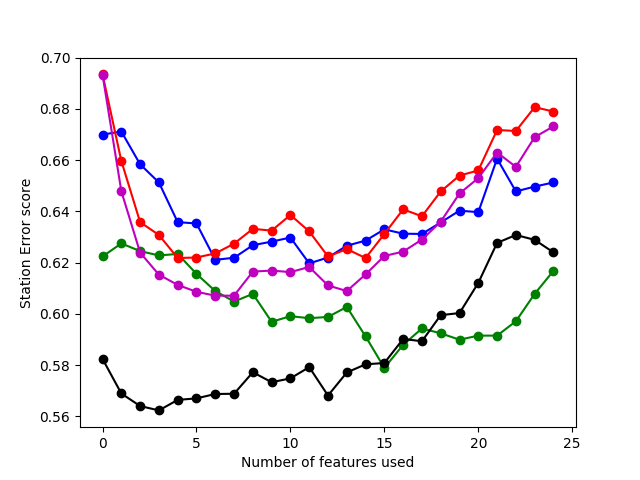
\includegraphics[clip,width=0.5\columnwidth]{fsstaerrs}}
\subfloat[System Error against number of variables seleted]{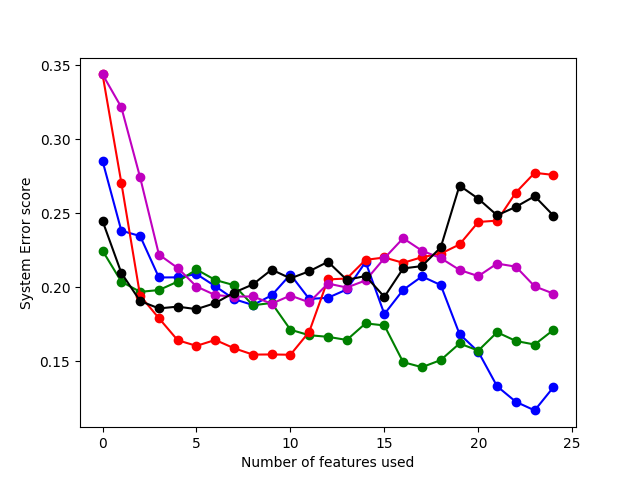
\includegraphics[clip,width=0.5\columnwidth]{fssyserrs}}
\captionsetup{singlelinecheck=off, font=scriptsize, justification=centering}
\caption[]{
Error against number of features used for stepwise forward selection\linebreak
Blue - Least Squares Linear; Green - Least Squares Log; Red - Poisson Log; Magenta - Poisson Identity; Black - LAD
%\begin{itemize}\setlength\itemsep{-5pt}
%\item Blue - Least Squares Linear
%\item Green - Least Squares Log
%\item Red - Poisson Log
%\item Magenta - Poisson Identity
%\item Black - Least Absolute Deviation
%\end{itemize}
}
\label{fig:bfscores}
\end{figure}

In general, each of the error scores decreases with the addition of new features up to a certain number of covariates, and then increases again. The minima for the system and station errors do not coincide with each other for any of the five regression methods, so there is a range of features which produce very similar error scores. By using the arithmetic average of the system and station errors, we pick an optimum number of features for each regression type; this is reported in Table \ref{tab:rresults}.  %In keeping with the optimization of LASSO on station-type loss functions, we will select as `best' the set of features that has the lowest station error. 

The station error is identical to the Least Absolute Deviation loss function. Therefore, it is not surprising that this regression type performs the best on the Station Error metric, having the lowest station error for up to 15 features. An interesting result of LAD regression is that the station error curve has its minimum much earlier than the other regression types, which show constant decreasing station error for at least the first six features. In the system error metric, the LAD regression loses its advantage. Instead, both the Least Squares regression methods produce low system error scores with increasing numbers of variables. 

The minimum scores from each regression type are recorded in Table \ref{tab:rresults} along with the average score over the range of good features. The stepwise regression significantly outperforms the LASSO regression in creating feature combinations that can accurately predict ridership in unknown transit networks. All the stepwise regression methods outperform all of the baseline methods showing the first block of the results table, in both error metrics. 

\subsection{Analysis of selected features}

A summary of selected features is given in Table \ref{tab:featuresum}. There are ten total regression methods used for feature selection; five LASSO methods and five forward selection methods. The count columns in Table \ref{tab:featuresum} shows the number of times each feature was selected by each regression method. For example, the \texttt{near\_hospitality} feature was selected by all ten methods, five LASSO and five forward selection.

The highly rated features display a mixture of potential correlation and causation with respect to transit ridership. For example, a major university is likely to drive transit ridership both in the immediately adjacent stations, and in nearby areas where students especially will live. On the other hand, the number of hospital jobs (\texttt{30net\_medical}) within 30 minutes of transit is more likely to be a reflection of population density rather than a driver of transit ridership. Some features, like the ubiquitously selected \texttt{near\_hospitality} are a mixture of both. Restaurants and hotels are likely to be located in areas of good transit accessibility, while they themselves will drive transit ridership to take advantage of their services. 

Because the forward selection models significantly outperformed the LASSO models, the variables chosen by the forward selection models are more likely to useful to a transit model. Conversely, there are several variables that were chosen by nearly all of the LASSO models, such as the number townhouses and duplexes within 15 minutes of a transit station (\texttt{15net\_hunits\_attached}) and the number of small apartment buildings within 15 minutes of a transit station (\texttt{15net\_hunits\_medium}). Since the LASSO methods performed worse than the baseline measures, it is likely that some of these variables actually decrease the performance of a model. 

Of the 94 features, 48 were not selected by any of the feature selection methods. Twenty-nine features were selected more than once, and fifteen were selected more than once by the forward selection models. 

\begin{table}[H]
\begingroup\fontsize{10}{15}\selectfont
\centering
\begin{tabular}{lccc}
\toprule
Feature Name&LASSO&Forward Selection&Total Count\\
\midrule
near\_hospitality&5&5&10\\
parking&4&3&7\\
near\_university&4&2&6\\
15net\_hunits\_old&2&3&5\\
30net\_medical&3&2&5\\
15net\_university&1&3&4\\
30net\_hunits\_large&2&2&4\\
near\_entertainment&2&2&4\\
15net\_hunits\_attached&4&0&4\\
15net\_hunits\_medium&4&0&4\\
30net\_entertainment&1&2&2\\
near\_hunits\_detached&1&2&3\\
near\_hunits\_old&1&2&3\\
near\_medical&1&2&3\\
near\_emp\_pay&2&1&3\\
near\_employment&2&1&3\\
near\_pop\_old&2&1&3\\
\end{tabular}
\caption{Features that were frequently selected by regression methodologies}\label{tab:featuresum}
\endgroup
\end{table}


\section{Conclusion and Future Work}\label{sec:acc}

Ultimately, the error scores for the forward selection models for all five regression variants in Table \ref{tab:rresults} are very similar. There is little evidence that one regression type is significantly more effective than any other. All five regression types are able to give system-wide ridership estimates within 20\% of the true value for identified sets of features. This error compares favorably with the 48\% average ridership prediction  error reported for 25 transportation networks in Flyvbjerg \cite{Flyvbjerg2006}, where Flyvjerg uses the same system error model identified in Section \ref{sec:metric}. 

In addition, this model produces ridership estimates based on information publicly available to citizens. A ridership model can be trained on public data from cities with transit systems in the United States. A city with no existing intra-urban rail transit system would only need to obtain zip-code level information available from the US Census Bureau's website to apply such a model to generate ridership estimates for a new construction rail system. 

The Mannheim-Florian four step model fundamentally depends on existing transit ridership information. For example, the starting point of a four step analysis for a new light rail line would be an existing bus line that runs a similar, hopefully identical, path. The advantage of this regression model is that it creates a new estimate from different sources, independent of any knowledge of the current system.

A model trained on the transit system of the six US cities included in this work, and using any of the five regression methods tested would be sufficiently accurate to justify use for validating new construction, system-wide cost estimates for urban rail transit in the United States. 

\subsection{Future Work}

Future work in on this model could proceed in two directions. The first direction is to continue improvement of the source data. This project used only zip code shapes to estimate counting features, since job and housing data was available only for the zip code, but the population features exist in more granular detail at the Census Tract level. The author generated exclusion zones which were designed to prevent job and people from being located in parks and water could be improved by incorporating detailed city land use maps. Finally, there is a major deficiency in source data because neither federal, state nor local government workers are included in the employment data sources used by the model. Of particular concern are university employment; university jobs within walking distance was a selected feature in five of the six models. Several large universities are located on the transit networks of this study and were not accounted for, such as University of Illinois at Chicago, University of Colorado--Denver, and University of Massachusetts--Boston. There are other cities not included in this study that have very large public universities, like Minneapolis, Austin, or Columbus. Under-representation of university jobs in these cities would negatively affect the validity of any estimates, especially given the importance of university related features in Table \ref{tab:featuresum}.

The second direction for future work is improvement of the model itself. The feature summary for this paper only analyzed whether or not a feature was selected by any of the LASSO or forward selection regression methods. There remains to be done an analysis of the magnitude and direction of each feature's coefficient, to ensure that frequently selected features are significant. A feature selected four times, but with coefficient magnitudes both positive and negative is not as significant as a selected feature that only has positive or negative coefficients. 

In this work, only $\ell_1$, LASSO regularization was used. However, the R package \texttt{glmnet} is capable of performing ElasticNet regression as well. ElasticNet \cite{Zou2005} is a linear mixture of the $\ell_1$ and $\ell_2$ penalties from the LASSO and ridge regression methods. For OLS and Poisson, a mixed regularization may be able to improve the performance of the feature selection. 


\pagebreak
\begin{appendices}

\section{Data sources}

\subsection{Ridership data}\label{app:ridership}
\begingroup
\fontsize{9}{10}\selectfont
\begin{tabular}{ll}
Los Angeles: & \url{http://libraryarchives.metro.net/DPGTL/Ridership/RailActivityByStationFY2014.xls} \\
Chicago:& \url{http://www.transitchicago.com/assets/1/ridership_reports/2015_Annual.pdf} \\
Atlanta:& \url{http://documents.atlantaregional.com/transportation/TFB_2014_v17.pdf}\\
Boston:& \url{http://archives.lib.state.ma.us/bitstream/handle/2452/266319/ocm18709282-2014.pdf} \\
Denver:& \url{http://www.rtd-denver.com/documents/serviced/lrt-activity-08-2015.pdf} and \\
& \url{http://www.rtd-denver.com/documents/serviced/lrt-activity-Jan-April-2016.pdf}\\
Dallas:& \url{https://www.dart.org/about/dartreferencebookmar16.pdf}\\
\end{tabular}
\endgroup

\subsection{US Census feature data sources}\label{app:features}

All feature data is accessed through the American Factfinder website at \url{factfinder.census.gov}.

\begingroup
\fontsize{9}{9}\selectfont
\begin{tabular}{ll}
Population&Table DP05, Item HC01\_VC03\\
Population, 18 and under&Table DP05, Item HC01\_VC03 - Item HC01\_VC32\\
Population, 65 and over&Table DP05, Item HC01\_VC37\\
Housholds&Table S1101, Item HC01\_EST\_VC02\\
Households with Children&Table S1101, Item HC01\_EST\_VC06\\
Families&Table S1101, Item HC01\_EST\_VC010\\
Population with at least Bachelors degree&Table S1701, Item HC01\_EST\_VC34\\
Population in labor force&Table S1701, Item HC01\_EST\_VC37\\
Employed population&Table S1701, Item HC01\_EST\_VC38\\
Full-time employed population&Table S1701, Item HC01\_EST\_VC47\\
Population living at greater than 500\% of poverty level&Table S1701, Item HC01\_EST\_VC56\\
Population living at less than 200\% of poverty level&Table S1701, Item HC01\_EST\_VC01 -  HC01\_EST\_VC59\\
Housing units&Table DP04, Item HC01\_VC03\\
Single-family detached housing units&Table DP04, Item HC01\_VC14\\
Housing units in duplexes or townhouses&Table DP04, Items HC01\_VC15 + HC01\_VC16\\
Housing units in structures of 3-9&Table DP04, Item HC01\_VC17 + HC01\_VC18\\
Housing units in structures of 10+&Table DP04, Item HC01\_VC19 + HC01\_VC20\\
Housing units built before 1940&Table DP04, Item HC01\_VC36\\
Housing units built after 2000&Table DP04, Item HC01\_VC27 + HC01\_VC28 + HC01\_VC29\\
Housing units occupied by owner&Table DP04, Item HC01\_VC65\\
Housing units occupied by renter&Table DP66\\
Number of Jobs&Table CB1500CZ11, Item ‘EMP’\\
Total pay of all jobs&Table CB1500CZ11, Item ‘PAYANN’\\
Number of jobs at hospitals&Table CB1500CZ21, NAICS code 622, Estimated\\
Number of jobs at universities&Table CB1500CZ21, NAICS code 6113, Estimated\\
Number of jobs in hospitalitiy field&Table CB1500CZ21, NAICS code 72, Estimated\\
Number of jobs in finance field&Table CB1500CZ21, NAICS code 52, Estimated\\
Number of jobs in professional fields&Table CB1500CZ21, NAICS code 54, Estimated\\
Number of jobs in entertainment fields&Table CB1500CZ21, NAICS code 71, Estimated\\
\end{tabular}
\endgroup

\end{appendices}

 
\bibliographystyle{unsrt}
\pagebreak\bibliography{bibrefs}





\end{document}